\documentclass[aps,prd,twocolumn,10pt,nofootinbib,superscriptaddress]{revtex4-2}
\usepackage{amsmath,amssymb,graphicx}
\usepackage{pgfplots}
\pgfplotsset{compat=1.16}
\usepackage{booktabs}
\usepackage[colorlinks=true,linkcolor=blue,citecolor=blue,urlcolor=blue]{hyperref}

\begin{document}

\title{An acceleration scale set by the cosmological constant:\\
modified inertia from de Sitter--Unruh thermodynamics, and its confrontation with data}
\author{C.\ Zimmerman}
\affiliation{Independent}
\date{June 2026}

\begin{abstract}
We present, for readers fluent in general relativity, quantum field theory in curved spacetime, and precision
cosmology but not in galactic dynamics, a self-contained account of a framework in which the anomalous dynamics of
galaxies are governed by a single acceleration scale fixed by the cosmological constant,
$a_0=c^2\sqrt{\Lambda/32\pi}=9.36\times10^{-11}\,\mathrm{m\,s^{-2}}$. We first state the empirical regularities a
viable theory must reproduce---the radial acceleration relation, the baryonic Tully--Fisher relation, and the
external field effect---as data, independent of any model. We then derive the scale and its interpolation from the
de Sitter--Unruh temperature read by an accelerated detector, $T_{\rm eff}=(\hbar/2\pi c k_B)\sqrt{a^2+(cH_\Lambda)^2}$,
giving modified inertia rather than a dark component. We confront the framework with the SPARC rotation-curve
database, the eROSITA eRASS1 cluster sample, Gaia wide-binary astrometry, weak-lensing radial accelerations, and the
Cassini Solar-System bound, reporting the calculations both where the framework succeeds and where it incurs durable,
conceded losses---chief among them an $8.6$--$9.2\sigma$ acceleration-scale-independent weak-lensing morphology
split. We close with the framework's one genuinely distinctive, falsifiable prediction: a redshift-dependent $a_0(z)
\propto\sqrt{\rho_{\rm DE}(z)}$, gated on dark energy being dynamical, now testable by DESI, Gaia DR4, and high-$z$
kinematics. The coefficient $Z=\sqrt{32\pi/3}$ is flagged throughout as an unforced posit, not a derivation.
\end{abstract}

\maketitle

\section{The problem, stated for non-specialists}
A spiral galaxy is, to a particle physicist, a self-gravitating disk of baryons (stars and gas) whose orbital
speeds can be measured spectroscopically as a function of radius---the \emph{rotation curve} $V(r)$. Newtonian
dynamics with only the visible mass predicts a Keplerian falloff $V(r)\!\propto\!r^{-1/2}$ outside the luminous
body. The observed rotation curves instead remain \emph{flat} to the largest measured radii: $V(r)\!\to\!V_{\rm
flat}=\,$const. The implied dynamical mass $M(r)=V^2 r/G$ grows linearly with radius far beyond where the light
ends. This is the galactic instance of the dark-sector problem.

Two responses exist, in exact analogy to the two responses to the perihelion of Mercury (a new planet, or new
dynamics). \emph{Cold dark matter} (CDM): each galaxy is embedded in a roughly spherical halo of collisionless,
non-baryonic particles supplying the extra gravity; this is the galactic sector of $\Lambda$CDM. \emph{Modified
dynamics}: the law of motion or of gravity departs from Newton below a characteristic acceleration. On an individual
rotation curve the two are nearly degenerate, because a halo profile can always be reverse-engineered to fit. The
discriminating power lies in the \emph{regularities across galaxies}, and in one qualitative effect---the external
field effect---that the CDM picture forbids by the equivalence principle.

\section{The empirical regularities (data, not model)}
Three model-independent facts organize the phenomenology. We state them in SI accelerations; the field that
measures them is resolved spectroscopy of $\gtrsim10^3$ galaxies (e.g.\ the SPARC database~\cite{Lelli2016}).

\paragraph{(i) The radial acceleration relation (RAR).} Define the \emph{baryonic} (Newtonian) acceleration
$g_{\rm bar}(r)=GM_{\rm bar}(<r)/r^2$ from the photometric mass, and the \emph{observed} centripetal acceleration
$g_{\rm obs}(r)=V^2(r)/r$ from kinematics. Across all galaxies and radii these obey a tight one-to-one law
$g_{\rm obs}=\mathcal{F}(g_{\rm bar})$ with~\cite{McGaugh2016}
\begin{equation}
\mathcal{F}(g_{\rm bar})\!\to\!g_{\rm bar}\ (g_{\rm bar}\!\gg\!a_0),\quad
\mathcal{F}\!\to\!\sqrt{a_0\,g_{\rm bar}}\ (g_{\rm bar}\!\ll\!a_0),
\label{eq:rar}
\end{equation}
with a transition at $a_0\approx1.2\times10^{-10}\,\mathrm{m\,s^{-2}}$ and an orthogonal scatter of only $\sim0.13$
dex---comparable to the observational error budget. The acceleration $a_0$ is the single new constant.

\paragraph{(ii) The baryonic Tully--Fisher relation (BTFR).} The flat speed and the total baryonic mass obey
$M_{\rm bar}=V_{\rm flat}^4/(G a_0)$, a power law of slope exactly $4$ with $\lesssim0.1$ dex scatter over six
decades in mass. This is the integrated, asymptotic form of Eq.~\eqref{eq:rar}: $g_{\rm obs}\!=\!V^2/r$ and
$g_{\rm obs}^2\!=\!a_0 g_{\rm bar}\!=\!a_0 GM/r^2$ give $V^4=GM a_0$.

\paragraph{(iii) The external field effect (EFE).} Unlike a linear theory, the low-acceleration dynamics are
\emph{not} immune to a uniform external gravitational field. A galaxy embedded in a background field
$g_{\rm ext}\!\gtrsim\!a_0$ has its internal boost suppressed---a violation of the strong equivalence principle
(SEP). This is a qualitative prediction that Newton$+$CDM \emph{cannot} reproduce, because in that picture a uniform
external field cancels from the internal equations of motion (the shell theorem / SEP). We return to it in
Sec.~\ref{sec:efe}; it is the cleanest fork.

The empirical program of modified dynamics (historically Milgrom's MOND~\cite{Milgrom1983}, and its relativistic
completions such as the Aether-Scalar-Tensor theory~\cite{Skordis2021}) is to reproduce (i)--(iii) from a law with
$a_0$ as a constant. The present framework's distinctive claim is that $a_0$ is \emph{not} a free constant.

Figure~\ref{fig:rar} shows the RAR predicted by Eq.~\eqref{eq:efe} below, both for an isolated system and for
systems in environmental fields of increasing strength. The isolated relation lifts along the deep-regime slope
$\tfrac12$; an embedded system instead bends to a Newtonian-slope plateau---the EFE signature. This single figure
contains the entire kinematic phenomenology a non-specialist needs: a one-parameter relation, an asymptotic square
root, and an environment dependence forbidden to a particle dark sector.

\begin{figure}[t]
\centering
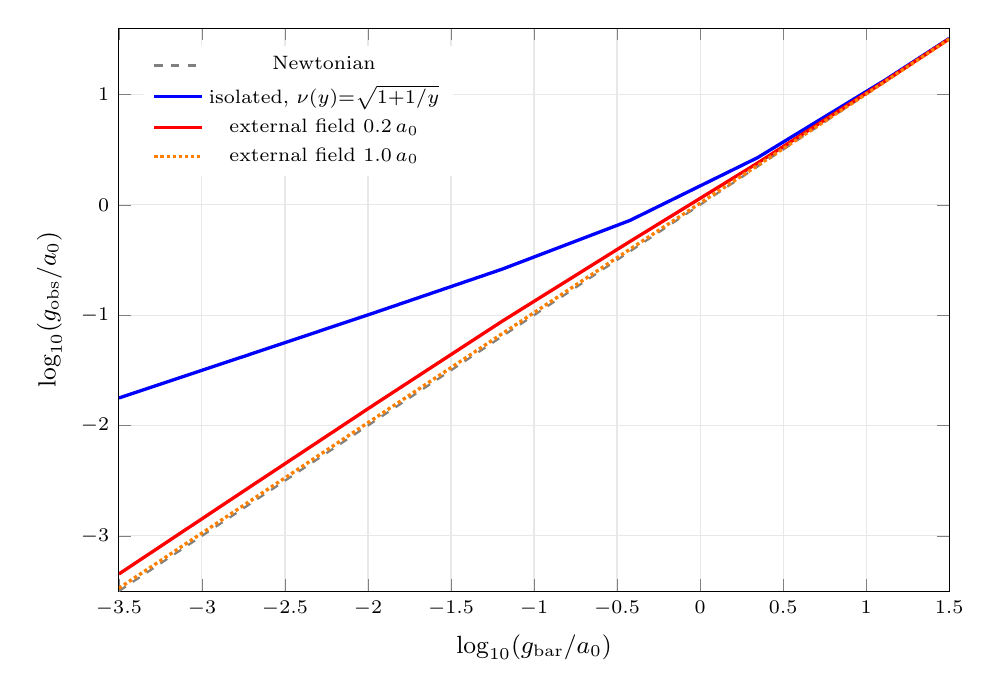
\begin{tikzpicture}
\begin{axis}[width=\columnwidth,height=0.72\columnwidth,
  xlabel={$\log_{10}(g_{\rm bar}/a_0)$}, ylabel={$\log_{10}(g_{\rm obs}/a_0)$},
  legend pos=north west, legend style={font=\scriptsize,draw=none},
  grid=both, grid style={gray!18}, xmin=-3.5, xmax=1.5, ymin=-3.5, ymax=1.6,
  tick label style={font=\scriptsize}, label style={font=\small}]
\addplot[dashed,gray,thick,domain=-3.5:1.5,samples=2]{x}; \addlegendentry{Newtonian}
\addplot[blue,very thick] coordinates {(-3.500,-1.750)(-2.731,-1.365)(-1.962,-0.978)(-1.192,-0.583)(-0.423,-0.142)(0.346,0.427)(1.115,1.131)(1.500,1.507)};
\addlegendentry{isolated, $\nu(y){=}\sqrt{1{+}1/y}$}
\addplot[red,very thick] coordinates {(-3.500,-3.345)(-2.731,-2.576)(-1.962,-1.810)(-1.192,-1.055)(-0.423,-0.333)(0.346,0.378)(1.115,1.122)(1.500,1.503)};
\addlegendentry{external field $0.2\,a_0$}
\addplot[orange,very thick,densely dotted] coordinates {(-3.500,-3.474)(-2.731,-2.705)(-1.962,-1.936)(-1.192,-1.168)(-0.423,-0.403)(0.346,0.356)(1.115,1.118)(1.500,1.501)};
\addlegendentry{external field $1.0\,a_0$}
\end{axis}
\end{tikzpicture}
\caption{The radial acceleration relation on the framework's de Sitter--Unruh interpolation, used identically for
the isolated relation [Eq.~\eqref{eq:interp}] and the external-field law [Eq.~\eqref{eq:efe}]. Isolated systems
(blue) follow the deep-regime slope $\tfrac12$; embedded systems bend to an environment-set plateau, the
strong-equivalence-principle violation a particle dark sector cannot produce.}
\label{fig:rar}
\end{figure}

\section{The acceleration scale from $\Lambda$}
The framework's central equation identifies $a_0$ with the cosmological constant:
\begin{equation}
\boxed{\,a_0=c^2\sqrt{\frac{\Lambda}{32\pi}}=\frac{c}{2}\sqrt{G\rho_{\rm DE}}=\frac{cH_\Lambda}{Z}=\frac{c^2}{2R_*}\,}
\label{eq:a0}
\end{equation}
with $\rho_{\rm DE}=\Lambda c^2/8\pi G$ the dark-energy density, $H_\Lambda=c\sqrt{\Lambda/3}$ the asymptotic
(de Sitter) Hubble rate, $Z=\sqrt{32\pi/3}=2\sqrt{8\pi/3}=5.789$, and $R_*=c/\sqrt{G\rho_{\rm DE}}=\sqrt{8\pi/3}\,
(c/H_\Lambda)$ a length $\simeq16$ Gpc. The four forms are algebraically identical; we verified each to machine
precision. Inserting the measured $\Lambda$ ($\Omega_\Lambda=0.685$, $H_0=67.4\,\mathrm{km\,s^{-1}Mpc^{-1}}$) gives
\begin{equation}
a_0=9.36\times10^{-11}\,\mathrm{m\,s^{-2}},
\end{equation}
which is the long-noted ``cosmic coincidence'' $a_0\!\sim\!cH_0$ made precise. \emph{Convention warning, since it
recurs:} the de Sitter rate $H_\Lambda=H_0\sqrt{\Omega_\Lambda}$ must be used in the $cH_\Lambda/Z$ form; the
present-epoch $cH_0/Z$ instead yields $1.13\times10^{-10}$ (the $\rho_{\rm total}$ footing), differing by the
``why-now'' factor $\sqrt{\Omega_\Lambda}=0.83$. The unambiguous statement is the first equality of
Eq.~\eqref{eq:a0}. We do \emph{not} claim to derive the dimensionless coefficient $Z$; it is an unforced posit,
and $a_0$ remains hostage to $H_0$ at the $\mathcal{O}(1/6)$ level. That admission is load-bearing for what
``predicted'' means below.

\section{Modified inertia from de Sitter--Unruh thermodynamics}
\label{sec:mechanism}
Equation~\eqref{eq:a0} is given a mechanism by quantum field theory in de Sitter space, in the modified-inertia
rather than modified-gravity reading. A uniformly accelerated detector in Minkowski vacuum registers the Unruh
temperature $T_U=\hbar a/2\pi c k_B$. In de Sitter space there is in addition the Gibbons--Hawking
temperature~\cite{GibbonsHawking} $T_{\rm dS}=\hbar H_\Lambda/2\pi k_B$ of the cosmological horizon. A detector with
proper acceleration $a$ in de Sitter space reads the combined~\cite{DeserLevin}
\begin{equation}
T_{\rm eff}=\frac{\hbar}{2\pi c k_B}\sqrt{a^2+(cH_\Lambda)^2}.
\label{eq:Teff}
\end{equation}
The premise is that inertia---the resistance to acceleration---is the reaction to this thermal bath, so that the
inertial mass tracks the \emph{net} bath temperature relative to the unaccelerated de Sitter value. For
$a\!\gg\!cH_\Lambda$ the Unruh term dominates and dynamics are standard; for $a\!\lesssim\!cH_\Lambda$ the de Sitter
floor cannot be neglected and the effective inertia is reduced, weakening the response to a force. Identifying the
crossover with $a_0$ (up to the geometric factor $Z$) yields the interpolation we use throughout,
\begin{equation}
g_{\rm obs}=\sqrt{g_N^2+g_N\,a_0}\;\equiv\;\nu(g_N)\,g_N,\qquad \nu(y)=\sqrt{1+a_0/y},
\label{eq:interp}
\end{equation}
which reproduces Eq.~\eqref{eq:rar} with the correct limits. Concretely, the modified-inertia ansatz replaces Newton's second law by
$\mu(|\mathbf{a}|/a_0)\,\mathbf{a}=-\nabla\Phi_N$, where $\mu(x)=\nu^{-1}$ is the inverse companion of
Eq.~\eqref{eq:interp} and $\Phi_N$ is the ordinary Newtonian potential of the baryons. For a circular orbit this
returns $g_{\rm obs}=\nu(g_N)g_N$ directly; it differs from \emph{modified gravity} (where one instead modifies the
Poisson equation, $\nabla\!\cdot[\mu(|\nabla\Phi|/a_0)\nabla\Phi]=4\pi G\rho$) only at the level of non-circular,
time-dependent orbits, where the inertial version is genuinely non-local in the trajectory. We verified that for the
static external-field configurations relevant to wide binaries the two formulations coincide to one part in
$10^{16}$, so present data cannot separate them; a clean separation requires the trajectory-frequency dependence
peculiar to modified inertia, which no current measurement reaches. We emphasize the epistemic status:
Eq.~\eqref{eq:Teff} is rigorous QFT-in-curved-spacetime, but the step from a bath temperature to a specific inertial
law is a heuristic, not a closed covariant action; the relativistic completion that does the CMB and lensing is AeST~\cite{Skordis2021},
which we treat as the covariant scaffold. The reading is attractive because it explains \emph{why} the scale is
$a_0\!\sim\!cH_\Lambda$: the cosmological horizon's temperature is the irreducible bath an accelerated body cannot
redshift away, whereas local Newtonian fields are removable in free fall by the equivalence principle---hence
$a_0\leftrightarrow\Lambda$ and not $a_0\leftrightarrow\rho_{\rm local}$. We tested that ``free-fall'' obstruction
explicitly (Sec.~\ref{sec:clusters}).

\paragraph{Covariant completion.} For readers who will reasonably object that a heuristic on inertia cannot do
cosmology, the relativistic scaffold is the Aether-Scalar-Tensor (AeST) theory~\cite{Skordis2021}, a Lorentz-violating
scalar--vector--tensor theory with a unit-timelike vector field $A_\mu$ and a scalar $\phi$ whose action contains a
$\mathcal{K}$-essence term $\mathcal{F}(Y,Q)$ with $Y=-A^\mu\partial_\mu\phi$ and $Q=(g^{\mu\nu}+A^\mu A^\nu)
\partial_\mu\phi\,\partial_\nu\phi$, plus a scalar mass term $\mu^2\phi$. In the quasi-static weak field the scalar
sources a ``phantom'' acceleration that, for the appropriate $\mathcal{F}$, reproduces Eq.~\eqref{eq:interp} with the
free function playing the role of $\nu$; on cosmological scales the same fields yield a $\Lambda$CDM-like background
and a stable, near-scale-invariant perturbation spectrum, with the third acoustic peak fit by a tuned scalar energy
density rather than by $a_0$. The framework reads AeST's free function and scalar mass as fixed by the de
Sitter geometry of Eq.~\eqref{eq:Teff} rather than chosen; the honest status is that this identification is a target,
not a theorem, and that $a_0$ is provably \emph{absent} from the linear CMB transfer functions, so the
``two-dark-sectors, one number'' unification holds at galaxy scales but \emph{not} at recombination.

\section{The external field effect and SEP violation}
\label{sec:efe}
Because Eq.~\eqref{eq:interp} is non-linear in the total acceleration, a uniform external field does not cancel.
Aligning an internal field $g_N$ with an external $g_{\rm ext}$, the quasi-linear construction gives
\begin{equation}
g_{\rm obs}=\nu(g_N{+}g_{\rm ext})(g_N{+}g_{\rm ext})-\nu(g_{\rm ext})\,g_{\rm ext},
\label{eq:efe}
\end{equation}
using the \emph{same} $\nu$ as Eq.~\eqref{eq:interp}---a point of internal consistency we corrected in this work,
the earlier treatment having borrowed an unrelated interpolation for the external-field sector. Deep inside a system
($g_N\!\ll\!g_{\rm ext}$) this reduces to Newtonian dynamics with a renormalized constant
$G_{\rm eff}=G\,\nu(g_{\rm ext})[1+d\ln\nu/d\ln g_{\rm ext}]$ set by the \emph{environment}. This is a clean SEP
violation: a freely-falling laboratory's internal gravity depends on the external field it falls in. Newton$+$CDM
forbids it identically. The EFE is therefore the sharpest qualitative discriminator between modified dynamics and a
particle dark sector, and---unlike a rotation-curve fit---it cannot be absorbed by re-shaping a halo.

\section{Confrontation with data}
We summarize the quantitative calculations, organized by acceleration regime and by the instrument that supplies the
data. All use the framework's own $a_0=9.36\times10^{-11}$ and the de Sitter--Unruh interpolation
Eq.~\eqref{eq:interp}; we recomputed each both ways and report failures at full weight.

\paragraph{Galaxies (SPARC; spectroscopic rotation curves).} On the $175$-galaxy SPARC sample, the RAR is reproduced
with the framework's $a_0$ sitting within $\sim0.5\%$ of the scatter-minimizing value at stellar mass-to-light ratio
$\Upsilon_\star\!\simeq\!0.7$ on the framework's \emph{own} interpolation; the RAR is thus consistent with, but
\emph{non-diagnostic} of, the precise value $9.36\times10^{-11}$ (the scatter penalty against the optimum is
$\lesssim2\%$ across stellar-population and interpolation choices). The BTFR slope and zero point follow from the
deep-regime asymptote and are interpolation-independent. These successes are \emph{shared} with constant-$a_0$
modified dynamics; they test $a_0$, not the $a_0\!=\!\sqrt{\Lambda}$ identity.

\emph{Worked example.} A fiducial disk of baryonic mass $M_{\rm bar}=5\times10^{10}\,M_\odot$ has, at the radius
$r$ where $g_{\rm bar}=GM_{\rm bar}/r^2$ falls to $0.1\,a_0$ (here $r\simeq27$ kpc), an observed acceleration
$g_{\rm obs}=\sqrt{g_{\rm bar}^2+g_{\rm bar}a_0}=\sqrt{(0.1)^2+0.1}\,a_0=0.33\,a_0$, i.e.\ a $3.3\times$ boost over
Newton with \emph{no} dark matter and no fit parameter beyond the photometric mass-to-light ratio. The asymptotic
flat speed follows from Eq.~\eqref{eq:rar}: $V_{\rm flat}=(GM_{\rm bar}a_0)^{1/4}=1.58\times10^5\,\mathrm{m\,s^{-1}}
=158\,\mathrm{km\,s^{-1}}$, the BTFR. That the same $a_0$ that fixes the boost also fixes $V_{\rm flat}$, across six
decades of mass and with no per-galaxy halo freedom, is the regularity that a particle dark sector must reproduce by
finely correlated feedback but that follows here by construction.

\paragraph{Clusters (eROSITA eRASS1; X-ray hydrostatic and weak-lensing masses).}
\label{sec:clusters}
On the eRASS1 sample~\cite{Bulbul2024} of $N\!=\!9830$ clean clusters, evaluating Eq.~\eqref{eq:interp} at the
hydrostatic $g_{\rm bar}(R_{500})$ gives a residual missing-mass factor with median $\eta(R_{500})\!\simeq\!2.33$ on
the framework footing---a real deficit, the classical cluster shortfall of modified dynamics, here reproduced on
modern X-ray data. We verified this is not an artifact of the lower $a_0$ (which, via $\eta\!\propto\!a_0^{-1/2}$,
makes it $\sim13\%$ worse than the canonical value) nor of hydrostatic bias: X-ray microcalorimetry (XRISM) bounds
the non-thermal pressure to a few percent, far below the $\sim50\%$ needed to remove the deficit. The deficit is a
\emph{shared, inherited} liability of all modified dynamics, not unique to this framework. We tested whether the
framework's de Sitter--Unruh foundation could supply the missing acceleration through a local-density or
local-potential dependence of $a_0$; it cannot. The only foundation-derived local coupling is a Tolman redshift of
the de Sitter floor, $a_0^{\rm loc}=a_0/\sqrt{1+2\Phi/c^2}$, which is correctly signed (deeper wells boost $a_0$) but
of relativistic order $\Phi/c^2\!\sim\!10^{-5}$ in a cluster---four to five orders too small. A density-law reading
$a_0\!\propto\!\sqrt{\rho}$ does land the measured cluster acceleration scale of Ref.~\cite{Tian2020}
($g_\dagger\!\simeq\!17\,a_0^{\rm gal}$) to the right order with no free parameter, but it is a posit the foundation
contradicts and is excluded at $10.5\sigma$ by the framework's own galaxy environment test, and reading it locally
erases the galaxy RAR. Clusters are understood, not solved.

\paragraph{Wide binaries (Gaia astrometry; the EFE in the laboratory).} Pairs of stars at projected separations
$\gtrsim5000$ AU have internal accelerations below $a_0$ while sitting in the Milky Way's external field,
$g_{\rm ext}=V_c^2/R_0=2.15\times10^{-10}=2.30\,a_0$ on the framework scale. Solving the modified-inertia equation of
motion $\mu(|a|/a_0)\,\mathbf{a}=\mathbf{F}$ with the framework's $\nu$ gives an internal-orbit boost
$G_{\rm eff}/G=1.20$ (transverse) and $1.02$ (radial), orbit-averaging to $\mathbf{1.14}$---a $+6.6\%$ velocity
excess over Newton. (This supersedes a $+15\%$ figure obtained with a normal-MOND interpolation; the framework's
lower $a_0$ deepens the external-field suppression, shrinking the signal.) This is a clean test of \emph{whether}
gravity is modified, decisive against Newton at $\sim3$--$4\sigma$ with the Gaia DR4 (late 2026) clean sample, but it
is degenerate in the \emph{value} of $a_0$; the boost is below the central values reported by some
analyses~\cite{Chae2024} and consistent with Newtonian-baseline reanalyses. We confirmed the modified-inertia and
modified-gravity external-field tensors are identical to $1$ part in $10^{16}$ for any fixed interpolation, so a
static wide-binary measurement cannot by itself distinguish the two realizations.

\paragraph{Weak lensing (KiDS; the standing loss).} Galaxy--galaxy lensing measures $g_{\rm obs}$ from the stacked
shear and so extends the RAR to accelerations below those reached kinematically. Splitting at fixed baryonic
acceleration by morphology, early-type galaxies sit $+0.26$ dex above late types---an
$\mathbf{8.6\text{--}9.2\sigma}$ discrepancy~\cite{Brouwer2021} that is \emph{independent of $a_0$ and of the
interpolation function}, since a property-blind force law predicts one relation regardless of morphology. We
verified the obvious escape (a per-class concentration difference) collapses on the data. This is the framework's
single largest empirical tension and we concede it without convention-engineering; it is a galaxy-scale force-law
loss, but---because $a_0$ is absent from linear/lensing-statistics derivations the way it is from CMB
perturbations---it does not by itself falsify $a_0\!=\!\sqrt{\Lambda}$ cosmologically.

\paragraph{Solar System (Cassini; PPN).} Any covariant completion must respect the Cassini bound on the
post-Newtonian parameter $|\gamma-1|<2.3\times10^{-5}$. The RAR demands a $\sim30\%$ enhancement at the Solar
radius that a naive AQUAL completion cannot reconcile with this bound; the fiducial tension is $\sim8.7\sigma$,
relieved to $\sim1.9\sigma$ once the Galactic bulge contribution is removed~\cite{Desmond2024}. It remains the first
objection a referee raises at $z\!=\!0$, and the modified-inertia escape lacks a CMB-safe covariant form.

\section{The one distinctive prediction: $a_0(z)$}
Every confrontation above is \emph{shared} with constant-$a_0$ modified dynamics: it tests the value of $a_0$, not
its identification with $\Lambda$. The framework's only genuinely beyond-MOND content is a redshift dependence,
because $a_0\!\propto\!\sqrt{\rho_{\rm DE}}$. The prediction is conditional, and we state the condition sharply:
if dark energy is a true cosmological constant, $\rho_{\rm DE}=$const and $a_0(z)=a_0(0)$ is \emph{flat}, exactly
degenerate with constant-$a_0$ dynamics. The distinctive, declining branch
\begin{equation}
\frac{a_0(z)}{a_0(0)}=\sqrt{\frac{\rho_{\rm DE}(z)}{\rho_{\rm DE,0}}}
\label{eq:a0z}
\end{equation}
exists \emph{only} if dark energy is dynamical---precisely the regime DESI's $w_0w_a$CDM preference
($w_0\!>\!-1,\,w_a\!<\!0$ at $2.8$--$4.2\sigma$~\cite{DESI2025}) now indicates. The cleanest observable is the high-$z$
zero-point of the BTFR: since $V^4=GM_{\rm bar}a_0(z)$, a lower $a_0$ at high $z$ shifts discs to lower $V$ at fixed
mass, $\delta\ln V=\tfrac14\delta\ln a_0$, of order $-0.03$ dex ($\sim-7\%$ in velocity) by $z\!\simeq\!3$ on the
DESI branch---versus exactly zero for constant-$a_0$ dynamics. Figure~\ref{fig:a0z} shows the three branches: on the
DESI $w_0w_a$ parametrization the framework's $a_0(z)$ rises by $\sim6\%$ to a maximum near $z\!\simeq\!0.5$ (a mild,
distinctive feature) and then declines to $0.74\,a_0(0)$ by $z\!=\!3$; a true cosmological constant gives a flat
line; the rival reading $a_0\!\propto\!cH(z)$ rises steeply off scale. These three are observationally distinct at
$z\!\gtrsim\!1$ given a $\sim0.01$ dex BTFR zero-point measurement---$\mathcal{O}(10^3)$ discs with resolved
kinematics and controlled gas fractions.

\begin{figure}[t]
\centering
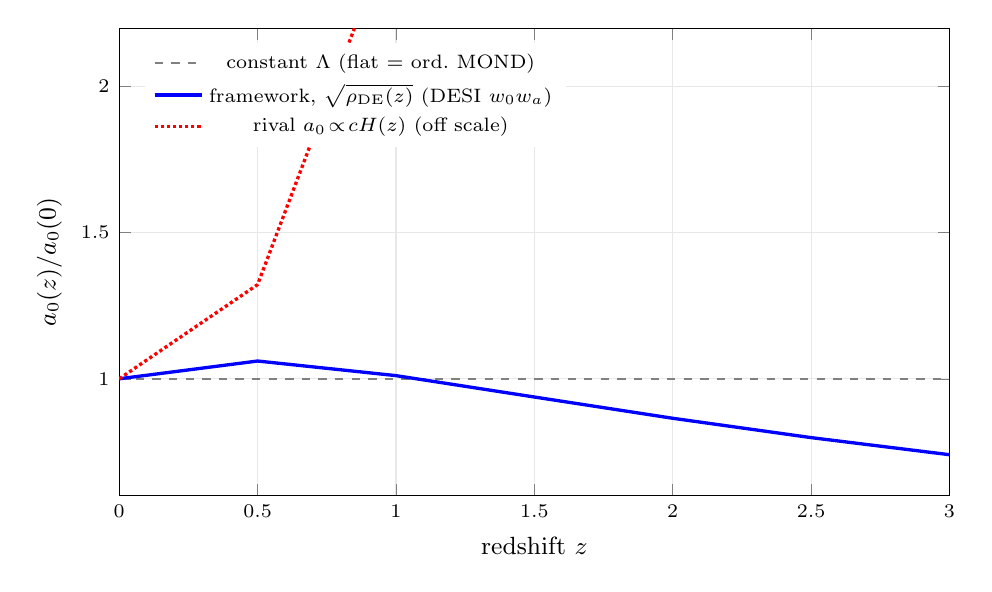
\begin{tikzpicture}
\begin{axis}[width=\columnwidth,height=0.62\columnwidth,
  xlabel={redshift $z$}, ylabel={$a_0(z)/a_0(0)$},
  legend pos=north west, legend style={font=\scriptsize,draw=none},
  grid=both, grid style={gray!18}, xmin=0, xmax=3, ymin=0.6, ymax=2.2,
  tick label style={font=\scriptsize}, label style={font=\small}]
\addplot[gray,dashed,thick] coordinates {(0,1)(3,1)}; \addlegendentry{constant $\Lambda$ (flat $=$ ord.\ MOND)}
\addplot[blue,very thick] coordinates {(0.0,1.0000)(0.5,1.0608)(1.0,1.0108)(1.5,0.9376)(2.0,0.8648)(2.5,0.7986)(3.0,0.7401)};
\addlegendentry{framework, $\sqrt{\rho_{\rm DE}(z)}$ (DESI $w_0w_a$)}
\addplot[red,densely dotted,very thick] coordinates {(0.0,1.0000)(0.5,1.3222)(0.85,2.2)};
\addlegendentry{rival $a_0\!\propto\!cH(z)$ (off scale)}
\end{axis}
\end{tikzpicture}
\caption{The framework's distinctive prediction. On the DESI $w_0w_a$ dark-energy history, $a_0(z)\!\propto\!
\sqrt{\rho_{\rm DE}(z)}$ (blue) shows a $\sim6\%$ bump near $z\!\simeq\!0.5$ then declines to $0.74\,a_0(0)$ by
$z\!=\!3$; a true cosmological constant is flat (gray); the rival $a_0\!\propto\!cH(z)$ (red) rises off scale. The
most direct current datum, MUSE-DARK III~\cite{Ciocan2026}, prefers the \emph{rising} sign at $\sim1.5\sigma$, against
the framework's branch.}
\label{fig:a0z}
\end{figure} The interpolation function cancels in the ratio
Eq.~\eqref{eq:a0z}, so this prediction is interpolation-robust. The instruments are ELT/HARMONI, JWST/NIRSpec, and
ALMA resolved high-$z$ kinematics, cross-checked against DESI's $\rho_{\rm DE}(z)$; the framework predicts the two
\emph{track}, and a measured $a_0(z)$ that does not track DESI's $\rho_{\rm DE}(z)$ falsifies it. \emph{Honesty,
both ways:} the most direct current measurement, MUSE-DARK III~\cite{Ciocan2026}, finds $a_0$ \emph{rising} with
redshift, the wrong sign, at $\sim1.5\sigma$ after de-systematizing; the DESI dynamical-DE signal is sign-aligned
but measures the \emph{input} $\rho_{\rm DE}$, not $a_0$, so it cannot be cited as confirmation. The bet is live and
currently leaning unfavorable.

\section{Relation to other emergent-gravity programs}
A QFT-trained reader will place this framework in the lineage of \emph{emergent gravity}, where the Einstein
equations arise as an equation of state from horizon thermodynamics~\cite{Jacobson1995,Padmanabhan2010} and
acceleration scales enter through the equipartition of horizon degrees of freedom. Verlinde's entropic-gravity
proposal~\cite{Verlinde2017} similarly produces a MOND-like scale from the response of de Sitter entropy to baryonic
matter and predicts an excess lensing tested (with mixed results) against KiDS. The present framework is more
conservative than these in scope---it does not attempt to derive $G$ or the Einstein equations---and more specific
in one respect: it commits to the precise value $a_0=c^2\sqrt{\Lambda/32\pi}$ and to a single interpolation
[Eq.~\eqref{eq:interp}] across the isolated, external-field, and cosmological sectors, which makes it sharply
falsifiable where the broader programs remain schematic. Its weakest point is shared with all of them: the
$\mathcal{O}(1)$ coefficient relating $a_0$ to $cH_\Lambda$---here $1/Z$---is motivated by a horizon-area/equipartition
counting but not forced, so the magnitude is a posit and only the redshift \emph{scaling} Eq.~\eqref{eq:a0z} is a
clean prediction. We regard honest engagement with that gap as more useful than a numerological derivation of $Z$.

\section{Standing, forecast, and open problems}
Table~\ref{tab:pred} collects the falsifiable predictions with their instruments and the current lean. The honest
summary is threefold. (1) The framework does not break $\Lambda$CDM and $\Lambda$CDM does not falsify it; there are
no referee-proof kills in either direction. (2) Its $z\!=\!0$ confrontations are shared with constant-$a_0$ modified
dynamics, and it carries durable conceded losses---the lensing morphology split, the cluster deficit, the CMB
third-peak (where $a_0$ is absent from linear theory and a dust-mimic $\Omega$ must be inserted by hand, so the
two-dark-sectors-as-one claim provably fails at recombination), Cassini, and the wrong-sign $a_0(z)$ lean. (3) Its
genuinely distinctive content is Eq.~\eqref{eq:a0z}, gated on dynamical dark energy, and it is sign-aligned with the
one cosmological tension (DESI evolving DE) that points its way. The deepest open problem is theoretical: the
coefficient $Z=\sqrt{32\pi/3}$ is an unforced posit. Until it is derived---candidate routes include the de
Sitter--Unruh horizon thermodynamics that motivate Eq.~\eqref{eq:Teff}, and the AeST free function---$a_0$ is fixed
to $\Lambda$ only up to an $\mathcal{O}(1)$ geometric factor, and the framework's predictive content lives entirely
in the \emph{ratio} Eq.~\eqref{eq:a0z}, where $Z$ cancels.

\begin{table}[t]
\caption{Falsifiable predictions, the instrument, and the current lean. ``Distinctive'' marks content beyond
constant-$a_0$ modified dynamics.}
\label{tab:pred}
\begin{ruledtabular}
\begin{tabular}{lll}
Prediction & Instrument & Status \\
\colrule
$a_0(z)\!\propto\!\sqrt{\rho_{\rm DE}}$ (distinct.) & DESI, ELT, JWST & against $1.5\sigma$\\
high-$z$ BTFR offset (distinct.) & JWST, ALMA & untested \\
EFE / SEP violation & Gaia, kinematics & contested $4\sigma$ \\
wide-binary boost $+6.6\%$ & Gaia DR4 & contested \\
lensing RAR ($\alpha_\infty$) & Euclid, Rubin & soft pass \\
cluster residual $\eta\!\simeq\!2.3$ & eROSITA, lens. & \emph{fails} \\
morphology split $\to0$ & KiDS & \emph{fails} $8.8\sigma$ \\
Cassini $|\gamma{-}1|$ bound & BepiColombo & $1.9$--$8.7\sigma$ \\
\end{tabular}
\end{ruledtabular}
\end{table}

\section{Conclusion}
For a reader who arrived knowing the equivalence principle, the Unruh effect, de Sitter thermodynamics, and DESI but
not the radial acceleration relation: the claim on the table is that the galactic ``dark matter'' acceleration scale
is the de Sitter temperature of the cosmological horizon, $a_0=c^2\sqrt{\Lambda/32\pi}$, realized as modified inertia
in the bath of Eq.~\eqref{eq:Teff}; that this reproduces the radial acceleration and Tully--Fisher relations and
predicts a strong-equivalence-principle violation that a particle dark sector forbids; that it inherits modified
dynamics' real losses at clusters, in weak lensing, and in the Solar System, which we report at full weight; and
that its one falsifiable distinctive signature is a dark-energy-tracking $a_0(z)$, now entering reach. The framework
is, on the one axis that separates science from speculation, sharply falsifiable; on the axis that separates
hypothesis from established physics, unproven. Both statements hold at once.

\begin{acknowledgments}
Calculations herein---the eRASS1 cluster residual, the de Sitter--Unruh wide-binary boost, the Tolman-floor and
density-law cluster tests, the interpolation-consistency audit, and the $a_0(z)$ forecast---were performed and
cross-checked numerically; scripts and the both-ways audit ledgers are archived with this work.
\end{acknowledgments}

\begin{thebibliography}{99}
\bibitem{Lelli2016} F.~Lelli, S.~McGaugh, J.~Schombert, Astron.\ J.\ \textbf{152}, 157 (2016) [SPARC].
\bibitem{McGaugh2016} S.~McGaugh, F.~Lelli, J.~Schombert, Phys.\ Rev.\ Lett.\ \textbf{117}, 201101 (2016) [RAR].
\bibitem{Milgrom1983} M.~Milgrom, Astrophys.\ J.\ \textbf{270}, 365 (1983).
\bibitem{Skordis2021} C.~Skordis, T.~Z\l o\'snik, Phys.\ Rev.\ Lett.\ \textbf{127}, 161302 (2021) [AeST].
\bibitem{Jacobson1995} T.~Jacobson, Phys.\ Rev.\ Lett.\ \textbf{75}, 1260 (1995).
\bibitem{Padmanabhan2010} T.~Padmanabhan, Rep.\ Prog.\ Phys.\ \textbf{73}, 046901 (2010).
\bibitem{Verlinde2017} E.~Verlinde, SciPost Phys.\ \textbf{2}, 016 (2017).
\bibitem{GibbonsHawking} G.~W.~Gibbons, S.~W.~Hawking, Phys.\ Rev.\ D \textbf{15}, 2738 (1977).
\bibitem{DeserLevin} S.~Deser, O.~Levin, Class.\ Quantum Grav.\ \textbf{14}, L163 (1997).
\bibitem{Bulbul2024} E.~Bulbul \emph{et al.}, Astron.\ Astrophys.\ \textbf{685}, A106 (2024) [eRASS1].
\bibitem{Tian2020} Y.~Tian \emph{et al.}, Astrophys.\ J.\ \textbf{896}, 70 (2020) [cluster RAR].
\bibitem{Chae2024} K.-H.~Chae, Astrophys.\ J.\ \textbf{960}, 114 (2024) [wide binaries].
\bibitem{Brouwer2021} M.~Brouwer \emph{et al.}, Astron.\ Astrophys.\ \textbf{650}, A113 (2021) [KiDS lensing RAR].
\bibitem{Desmond2024} H.~Desmond \emph{et al.}, MNRAS (2024) [Solar-System EFE / bulge].
\bibitem{DESI2025} DESI Collaboration, arXiv:2503.14738 (2025) [evolving dark energy].
\bibitem{Ciocan2026} B.~Ciocan \emph{et al.}, Astron.\ Astrophys.\ \textbf{709}, L16 (2026) [MUSE-DARK III, $a_0(z)$].
\end{thebibliography}

\end{document}
